\documentclass{article}
\usepackage[utf8]{inputenc}
\usepackage[T1]{fontenc}
\usepackage{ngerman}
\usepackage{amsmath}
\usepackage{amsfonts}
\usepackage{a4wide}
\usepackage{color}
\usepackage{colortbl}
\usepackage{graphicx}
\definecolor{rose}{rgb}{1, 0.57, 0.69}		      
		      
\title{Praktikum Multicore-Programmierung \\ Abschlussprojekt 1}
\author{Gruppe 3: Sarah Lutteropp und Johannes Sailer}

\date{\today}
% Hinweis: \title{um was auch immer es geht}, \author{wer es auch immer 
% geschrieben hat} und  \date{wann auch immer das war} k\"onnen vor 
% oder nach dem  Kommando \begin{document} stehen 
% Aber der \maketitle Befehl mu\ss{} nach dem \begin{document} Kommando stehen! 
\begin{document}

\maketitle


\begin{abstract}
Dies ist eine Ausarbeitung für das Abschlussprojekt des Praktikums Multicore-Programmierung im Wintersemester 2015/16. Ziel des Projektes war es, am Beispiel des Jacobi-Verfahrens und des Gauß-Seidel-Verfahrens parallele Lösungsmethoden partieller Differentialgleichungen zu implementieren.
\end{abstract}

\section{Mathematischer Hintergrund}

%Wir haben folgendes Setting:
%\begin{itemize}
%	\item $\Omega \cup \Gamma = [0,1]^2$
%	\item Rand $\Gamma = \{(x,y) \in \mathbb{R}^2 : x \in \{0,1\} \text{ oder }  y \in \{0,1\} \}$
%	\item $-\Delta u(x,y) = f(x,y) \quad \forall (x,y) \in (0,1)^2$
%	\item $u(x,y) = 0 \quad \forall (x,y) \in [0,1]^2 \backslash (0,1)^2$
%	
%	\item Diskretisierungsparameter $h$
%	\item $(x,y)$ sind also Koordinaten im diskretisierten Einheitsquadrat
%	\item Vereinfachte Schreibweise: $u_{i,j} = u(x_i, y_j) \in \mathbb{R}$
%	\item $n$ ist die Anzahl der Gitterpunkte pro Dimension
%	\item Im Vektor $u^k \in \mathbb{R}^{n^2}$ stehen die Werte von $u$ für alle Gitterpunkte im Iterationsschritt $k$. Diese Notation ist echt doof, weil man das ständig mit der Funktion $u$ selbst verwechselt. :-(
%\end{itemize}

Anhand des Beispiels der Approximation von Stoffkonzentrationen innerhalb eines festgelegten zweidimensionalen durch ein Gitter angenäherten Gebietes ergibt sich mittels der auf dem Aufgabenblatt dargestellten Umformungen, Randbedingungen und Argumentationsschritte das lineare Gleichungssystem $Au = b$, das wir mittels Iterationsverfahren lösen sollen.

Hierbei ist
$A = \begin{pmatrix}
T & -I &  &  &  \\ 
-I & T & -I &  &  \\ 
 & \ddots & \ddots & \ddots &  \\ 
 &  & -I & T & -I \\ 
 &  &  & -I & T \\ 
\end{pmatrix} \in \mathbb{Z}^{2n \times 2n}, \quad$
$T \in \mathbb{Z}^{TODO \times TODO}$ 

mit $T_{i,j} = \begin{cases} 4 & \text{falls } i = j \\ -1 & \text{falls } |i-j| = 1 \\ 0 & \text{sonst}\end{cases}, \quad$ 
$u = \begin{pmatrix}
u_{1,1} \\ 
\vdots \\
u_{n,n}
\end{pmatrix} \text{ und } b = h^2 * \begin{pmatrix}
f(x_1, y_1) \\ 
\vdots \\
f(x_n, y_n)
\end{pmatrix}.$

Es ist $h \leq 1$, $\frac{1}{h} \in \mathbb{N}$, $n = \frac{1}{h}-1$, $x_i = y_i = h*i$ für $i = 1, \ldots, n$ und $f : \mathbb{R} \to \mathbb{R}$ eine Funktion. Bei $I$ handelt es sich um die $TODO \times TODO$-Einheitsmatrix.

~\\

Für $h = \frac{1}{3}$ ergibt sich beispielsweise das folgende Gleichungssystem:

$$\begin{pmatrix}
4 & -1 & -1 & 0 \\ 
-1 & 4 & 0 & -1 \\ 
-1 & 0 & 4 & -1 \\ 
0 & -1 & -1 & 4
\end{pmatrix} *
\begin{pmatrix}
u_{1,1} \\ 
u_{1,2} \\ 
u_{2,1} \\ 
u_{2,2}
\end{pmatrix} = \left(\frac{1}{3}\right)^2 *
\begin{pmatrix}
f(1/3,1/3) \\ 
f(1/3,2/3) \\ 
f(2/3,1/3) \\ 
f(2/3,2/3)
\end{pmatrix}
$$

Man könnte dieses lineare Gleichungssystem natürlich auch mit direkten Verfahren wie dem Gaußschen-Eliminationsverfahren lösen. Dieses ist jedoch nur sehr schlecht parallelisierbar. Außerdem ist das Gaußsche-Eliminationsverfahren sehr anfällig für numerische Störungen. Das ist bei iterativen Verfahren normalerweise nicht der Fall.

TODO: Überführung auf zweidimensionales Problem, den Lösungsvektor $u$ als Lösungsmatrix $U$ uminterpretieren.


\subsection{Jacobi-Verfahren}
Blabla
\subsubsection{Herleitung}
Blabla
\subsubsection{Abbruchkriterium} \label{jacobi:abbruch}
Unser Abbruchkriterium nimmt von allen Matrix Einträgen die Differenz zum neuen Punkt und summiert die Beträge davon auf. Dies schien uns recht Performant zu sein und da es auch in der Vorlesung Heterogene Parallele Rechensysteme Verwendung findet sollte es nicht so schlecht sein. Es werden auch keine Sprünge oder ähnliches verwendet, von demher ist der Overhead konstant.\\
Zur Auswahl standen außerdem das selbe wie oben in der euklidischen Norm zu berechnen, jedoch erschien uns oberes schneller.
Desweiteren dachten wir an den Vergleich der Veränderung der Hauptdiagonalelemente, was in einem zusätzlichen if geendet hätte.
Dann gab es noch eine Version mit Eigenwerten, welche wir nicht haben, was sich dadurch erledigt hatte.
\subsection{Gauß-Seidel-Verfahren}
Blabla
\subsubsection{Herleitung}
Blabla
\subsubsection{Abbruchkriterium}
Für das Gauß-Seidel-Verfahren haben wir dasselbe Abbruchkriterium wie in Abschnitt~\ref{jacobi:abbruch} verwendet. (TODO: Begründung)

\subsection{Vergleich der Konvergenz und Stabilität beider Verfahren}\label{konvergenz}
\begin{figure}[htbp] 
  \centering
     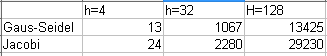
\includegraphics[width=0.7\textwidth]{bilder/convergenz.png}
  \caption{Beide Verfahren für verschiedene Verfeinerungen, bis das Abbruchkriterium true wurde.}
  \label{fig:Bild1}
\end{figure}

\section{Sequentielle Implementierung}

Die Matrixeinträge werden in dem auf dem Aufgabenblatt zur Verfügung gestellten Pseudocode spaltenweise durchlaufen. Daher haben wir in unserer Implementierung die Matrizen spaltenweise indiziert, um eine möglichst gute Cache-Lokalität zu erzielen.

Anstatt des Parameters $h$ übergeben wir einen Parameter $size$, der $\frac{1}{h}+1$ entspricht. Dies hat den Vorteil, dass der Nutzer den Grad der Verfeinerung exakt ohne Gleitkommaungenauigkeiten angeben kann und $U$ eine $size \times size$-Matrix ist.
 
Da sich die Einträge des Vektors $b$ innerhalb der Iterationen nicht ändern, haben wir $b$ vorberechnet.

\subsection{Laufzeiten bei verschiedenen Verfeinerungen}
Blabla
\subsection{Approximationsfehler}
Wir haben den Approximationsfehler nur für h=4 und h=32 dargestellt, weil Open Office nicht genug Punkte verarbeiten kann.
\begin{figure}[htbp] 
  \centering
     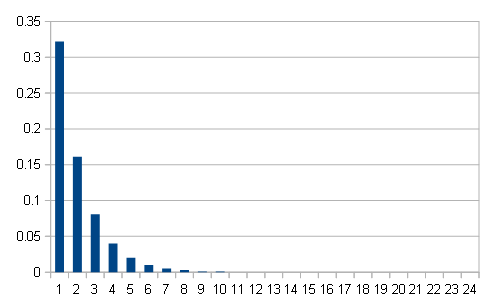
\includegraphics[width=1\textwidth]{bilder/dj4.png}
  \caption{Jacobi Approximationsfehler für h=4}
  \label{fig:Bild1}
\end{figure}
\begin{figure}[htbp] 
  \centering
     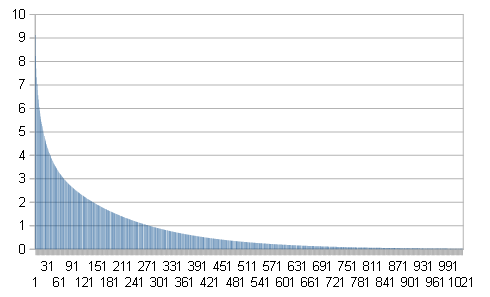
\includegraphics[width=1\textwidth]{bilder/dj32.png}
  \caption{Jacobi Approximationsfehler für h=32}
  \label{fig:Bild1}
\end{figure}

\begin{figure}[htbp] 
  \centering
     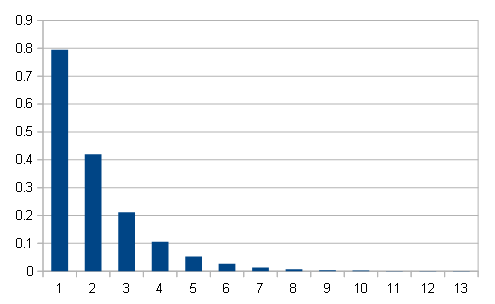
\includegraphics[width=1\textwidth]{bilder/dgs4.png}
  \caption{Gaus-Seidel Approximationsfehler für h=4}
  \label{fig:Bild1}
\end{figure}
\begin{figure}[htbp] 
  \centering
     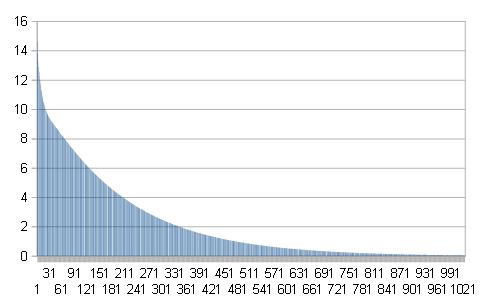
\includegraphics[width=1\textwidth]{bilder/dgs32.png}
  \caption{Gaus-SeidelApproximationsfehler für h=32}
  \label{fig:Bild1}
\end{figure}
\section{Parallelisierung}
Blabla
\subsection{Jacobi-Verfahren} \label{parallel:jacobi}
Da innerhalb der Iterationsschritte des Jacobi-Verfahrens keinerlei Datenabhängigkeiten bei der Berechnung der Matrixeinträge bestehen, haben wir mittels OpenMP (\texttt{\#pragma omp parallel for}) die äußere Schleife parallelisiert.

Zudem haben wir eine weitere Version des Jacobi-Verfahrens implementiert, in der wir zusätzlich zur Parallelisierung der \texttt{for}-Schleife auch den Code innerhalb der \texttt{for}-Schleife mit SSE vektorisiert haben.

Hierbei haben wir folgenden Speedup bei verschiedenen Problemgrößen $h$ und sowie verschiedenen Prozessorzahlen $p$ gemessen: TODO

\subsection{Gauß-Seidel-Verfahren}

Innerhalb der Iterationsschritte des Gauß-Seidel-Verfahrens bestehen Datenabhängigkeiten, da die Berechnung der Matrixeinträge in einer Iteration von den vorher berechneten Einträgen der selben Iteration abhängt. Das Gauß-Seidel-Verfahren ist daher inhärent sequentiell. Daher ist eine Parallelisierung des Gauß-Seidel-Verfahrens mit mehr Aufwand verbunden als beim ``embarassingly parallel'' Jacobi-Verfahren.

Wir haben sowohl den naiven, falschen Parallelisierungsansatz als auch zwei verschiedene funktionierende Parallelisierungsansätze implementiert.

\subsubsection{Naiver Parallelisierungsansatz}\label{gs:naiv}
Der naive Parallelisierungsansatz ist, wie in Abschnitt~\ref{parallel:jacobi} die äußerste Schleife mittels \texttt{\#pragma omp parallel for} zu parallelisieren. Da eine parallele Ausführung der Schleifeniterationen mittels OpenMP nicht die Iterationsreihenfolge garantiert, kann es hierbei zu Wettlaufsituationen (``Race Conditions'') kommen.

Im Fall des Gauß-Seidel-Verfahrens tritt dies in folgendem Beispiel auf (TODO: Beispiel):


Der im Praktikum vorgestellte Intel Thread Sanitizer erkennt die auftretende Wettlaufsituation nicht.

%\newpage
\subsubsection{Erweiterter Parallelisierungsansatz: Rot-Schwarz}

Bei der Rot-Schwarz-Parallelisierung des Gauß-Seidel-Verfahrens wird ausgenutzt, dass jeder Matrixeintrag nur von seinem linken, rechten, oberen und unteren direkten Nachbarn abhängt. Wir färben also die Matrixeinträge in rote und schwarze Felder ein, wobei die Datenabhängigkeiten nur zwischen Einträgen unterschiedlicher Farbe bestehen. Hierbei ergibt sich ein Schachbrettmuster, wie in Abbildung~\ref{fig:matrix} gezeigt.

\begin{figure}[h!]
\centering
$$U = 
\begin{tabular}{cccccc}
  \cellcolor{rose} & \cellcolor[gray]{0.7} & \cellcolor{rose} & \cellcolor[gray]{0.7} & \cellcolor{rose} & \cellcolor[gray]{0.7}\\
 \cellcolor[gray]{0.7} & \cellcolor{red} & \cellcolor[gray]{0.45} & \cellcolor{red} & \cellcolor[gray]{0.45} & \cellcolor{rose}\\
  \cellcolor{rose} & \cellcolor[gray]{0.45} & \cellcolor{red} & \cellcolor[gray]{0.45} & \cellcolor{red} & \cellcolor[gray]{0.7}\\
 \cellcolor[gray]{0.7} & \cellcolor{red} & \cellcolor[gray]{0.45} & \cellcolor{red} & \cellcolor[gray]{0.45} & \cellcolor{rose} \\
 \cellcolor{rose} & \cellcolor[gray]{0.45} & \cellcolor{red} & \cellcolor[gray]{0.45} & \cellcolor{red} & \cellcolor[gray]{0.7}\\
 \cellcolor[gray]{0.7} & \cellcolor{rose} & \cellcolor[gray]{0.7} & \cellcolor{rose} & \cellcolor[gray]{0.7} & \cellcolor{rose}\\
\end{tabular}
$$
\caption{Aufteilung der Lösungsmatrix $U$ in rote und schwarze Zellen, sodass zwischen Zellen gleicher Farbe keine Datenabhängigkeiten bestehen. Die Randzellen, deren Einträge per Annahme immer den Wert $0$ enthalten, sind in blasseren Farben markiert.}
\label{fig:matrix}
\end{figure}

Da die Matrixeinträge gleicher Farbe nicht voneinander abhängen, können wir diese parallel berechnen. Dies führt zu folgendem Ansatz: (TODO: Pseudocode)

Hierbei ist zu beachten, dass die einzelnen Iterationen des sequentiellen Gauß-Seidel-Verfahrens und dessen Rot-Schwarz-Parallelisierung nicht genau dasselbe Ergebnis liefern. Dies liegt darin begründet, dass durch die Rot-Schwarz-Aufteilung eine Umordnung der Matrixeinträge geschieht.

Um die Indexberechnung zu vereinfachen und die Cachelokalität zu verbessern, haben wir die roten und die schwarzen Einträge jeweils in eigenen, neuen Matrizen gespeichert. Dadurch liegen Einträge gleicher Farbe zusammenhängend im Speicher. Dies hat es uns auch ermöglicht, unsere Implementierung mittels SSE-Vektorinstruktionen zu beschleunigen. Die Vektorisierung mittels SIMD-Instruktionen haben wir explizit implementiert. Zwar ist mit OpenMP 4.0 eine Vektorisierung von Code auch mittels \texttt{\#pragma omp simd} möglich, aber unser händisch vektorisierter Code war schneller als der von OpenMP generierte.

Bei den Indexberechnungen haben wir zwischen $size \times size$-Matrizen gerader und ungerader $size$ unterschieden.

\paragraph{Berechnung der Nachbarindizes für gerade Werte von $size$}~\\
Für rote $U_{i,j}$ gilt: Der zugehörige Index in der Matrix für die roten Einträge ist $idx = \lfloor\frac{i+j*size}{2}\rfloor$. Der linke Nachbar ist an Stelle $idx - \frac{size}{2}$ in der Schwarz-Matrix. Der obere Nachbar ist an Stelle $idx - (1-(j \mod 2))$ in der Schwarz-Matrix. Der rechte Nachbar ist an Stelle $idx + \frac{size}{2}$ in der Schwarz-Matrix. Der untere Nachbar ist an Stelle $idx + (j \mod 2)$ in der Schwarz-Matrix.



Für schwarze $U_{i,j}$ gilt: Der zugehörige Index in der Matrix für die schwarzen Einträge ist $idx = \lfloor\frac{i+j*size}{2}\rfloor$. Der linke Nachbar ist an Stelle $idx - \frac{size}{2}$ in der Rot-Matrix. Der obere Nachbar ist an Stelle $idx - (j \mod 2)$ in der Rot-Matrix. Der rechte Nachbar ist an Stelle $idx + \frac{size}{2}$ in der Rot-Matrix. Der untere Nachbar ist an Stelle $idx + (1- (j \mod 2))$ in der Rot-Matrix.

Abbildung~\ref{fig:matrix:even} zeigt die Berechnung der Nachbarindizes am Beispiel $size=6$.

\begin{figure}[h!]
\centering
$$U = 
\begin{tabular}{cccccc}
  \cellcolor{rose}0 & \cellcolor[gray]{0.7}3 & \cellcolor{rose}6 & \cellcolor[gray]{0.7}9 & \cellcolor{rose}12 & \cellcolor[gray]{0.7}15\\
  
 \cellcolor[gray]{0.7}0 & \cellcolor{red}3 & \cellcolor[gray]{0.45}6 & \cellcolor{red}9 & \cellcolor[gray]{0.45}12 & \cellcolor{rose}15\\
 
  \cellcolor{rose}1 & \cellcolor[gray]{0.45}4 & \cellcolor{red}7 & \cellcolor[gray]{0.45}10 & \cellcolor{red}13 & \cellcolor[gray]{0.7}16\\
  
 \cellcolor[gray]{0.7}1 & \cellcolor{red}4 & \cellcolor[gray]{0.45}7 & \cellcolor{red}10 & \cellcolor[gray]{0.45}13 & \cellcolor{rose}16 \\
 
 \cellcolor{rose}2 & \cellcolor[gray]{0.45}5 & \cellcolor{red}8 & \cellcolor[gray]{0.45}11 & \cellcolor{red}14 & \cellcolor[gray]{0.7}17\\
 
 \cellcolor[gray]{0.7}2 & \cellcolor{rose}5 & \cellcolor[gray]{0.7}8 & \cellcolor{rose}11 & \cellcolor[gray]{0.7}14 & \cellcolor{rose}17\\
\end{tabular} \quad
$$
\caption{Berechnung der Nachbarindizes für gerade Werte von $size$ am Beispiel $size=6$}
\label{fig:matrix:even}
\end{figure}

\paragraph{Berechnung der Nachbarindizes für ungerade Werte von $size$}~\\
Für rote $U_{i,j}$ gilt: Der zugehörige Index in der Matrix für die roten Einträge ist $idx = \lfloor\frac{i+j*size}{2}\rfloor$. Der linke Nachbar ist an Stelle $idx - \lceil\frac{size}{2}\rceil$ in der Schwarz-Matrix. Der obere Nachbar ist an Stelle $idx - 1$ in der Schwarz-Matrix. Der rechte Nachbar ist an Stelle $idx + \lfloor\frac{size}{2}\rfloor$ in der Schwarz-Matrix. Der untere Nachbar ist an Stelle $idx$ in der Schwarz-Matrix.



Für schwarze $U_{i,j}$ gilt: Der zugehörige Index in der Matrix für die schwarzen Einträge ist $idx = \lfloor\frac{i+j*size}{2}\rfloor$. Der linke Nachbar ist an Stelle $idx - \lfloor\frac{size}{2}\rfloor$ in der Rot-Matrix. Der obere Nachbar ist an Stelle $idx$ in der Rot-Matrix. Der rechte Nachbar ist an Stelle $idx + \lceil\frac{size}{2}\rceil$ in der Rot-Matrix. Der untere Nachbar ist an Stelle $idx + 1$ in der Rot-Matrix.

Abbildung~\ref{fig:matrix:odd} zeigt die Berechnung der Nachbarindizes am Beispiel $size=7$.

\begin{figure}[h!]
\centering
$$U = 
\begin{tabular}{ccccccc}
  \cellcolor{rose}0 & \cellcolor[gray]{0.7}3 & \cellcolor{rose}7 & \cellcolor[gray]{0.7}10 & \cellcolor{rose}14 & \cellcolor[gray]{0.7}17 & \cellcolor{rose}21 \\
  
 \cellcolor[gray]{0.7}0 & \cellcolor{red}4 & \cellcolor[gray]{0.45}7 & \cellcolor{red}11 & \cellcolor[gray]{0.45}14 & \cellcolor{red}18 & \cellcolor[gray]{0.7}21\\
 
  \cellcolor{rose}1 & \cellcolor[gray]{0.45}4 & \cellcolor{red}8 & \cellcolor[gray]{0.45}11 & \cellcolor{red}15 & \cellcolor[gray]{0.45}18 & \cellcolor{rose}22\\
  
 \cellcolor[gray]{0.7}1 & \cellcolor{red}5 & \cellcolor[gray]{0.45}8 & \cellcolor{red}12 & \cellcolor[gray]{0.45}15 & \cellcolor{red}19 & \cellcolor[gray]{0.7}22\\
 
 \cellcolor{rose}2 & \cellcolor[gray]{0.45}5 & \cellcolor{red}9 & \cellcolor[gray]{0.45}12 & \cellcolor{red}16 & \cellcolor[gray]{0.45}19 & \cellcolor{rose}23\\
 
 \cellcolor[gray]{0.7}2 & \cellcolor{red}6 & \cellcolor[gray]{0.45}9 & \cellcolor{red}13 & \cellcolor[gray]{0.45}16 & \cellcolor{red}20 & \cellcolor[gray]{0.7}23\\
 
 \cellcolor{rose}3 & \cellcolor[gray]{0.7}6 & \cellcolor{rose}10 & \cellcolor[gray]{0.7}13 & \cellcolor{rose}17 & \cellcolor[gray]{0.7}20 & \cellcolor{rose}24 \\
\end{tabular} \quad
$$
\caption{Berechnung der Nachbarindizes für ungerade Werte von $size$ am Beispiel $size=7$}
\label{fig:matrix:odd}
\end{figure}

\newpage

\paragraph{Messung von Speedup und Effizienz unter verschiedenen Verfeinerungen, Skalierbarkeit}
TODO

\subsubsection{Erweiterter Parallelisierungsansatz: Wavefront}
Beim Wavefront Algorithmus wird anstatt über die  Spalten oder Zeilen zu iterieren über die Diagonalen iteriert. Das hat den Vorteil, dass die Daten nicht voneinander abhängig sind und das selbe herauskommt, wie beim eigentlichen Gaus-Seidel Verfahren in serieller Form.

Vermutlicher Grund wieso unsere Wavefront-Implementierung langsamer als sequentielles Gauß-Seidel: Die Indexberechnung ist sehr aufwändig. Wir berechnen  die Indizes in jeder Iteration neu, anstatt sie einmalig vorzuberechnen und in einer ``Indextabelle'' zu speichern. Außerdem richtet sich die Parallelität nach der Anzahl der Diagonal Elemente. D.h. es lohnt sich erst bei großen Diagonalen.

Bei der Wavefront Cache Lösung, wurden die Matrix zu erst in einen anderen Array kopiert, indem die Diagonalen in den Zeilen stehen. Dadurch haben wir uns erhofft, dass es zu einer höheren Cache Hitrate kommt. \\
In beiden Wavefront Lösungen hätte man sicher noch einiges optimieren können(z.B. Cuda für große Diagonalen), jedoch erschien uns Rot-Schwarz so viel schneller, dass es sich nicht lohnen würde.

\paragraph{Berechnung der Indexe}
Für die Implementierung wurden drei Schleifen verwendet. die Äußere ist zwischen den Schritten des Gaus-Seidel verfahren, die mittlere geht über die Diagonalen und die innere über die Elemente der Diagonalen. \\
In der Mittleren schleife werden die Variablen für die aktuelle Anzahl an Elementen gesteuert sowie eine Variable die angibt in welchem Durchlauf man nach der Diagonalen ist(border). Diese dient dazu anzugeben, wie viele Elemente man am Rand weg lassen kann, weil sie nicht mehr in der Matrix sind.\\
Bei der Wavefront Cache Lösung muss bei jeder Indexberechnung die Eingangspermutation, welche die Diagonalen den Zeilen des Arrays zuweist umkehren um die Indexe zu berechnen. Hierbei möchte ich auf die grandios  benannten Variablen hack und hack2 eingehen. Diese werden benutzt um die Elemente um das zu berechnende Element zu adressieren. hack wird 1 Durchgang vor der Diagonalen zu 1, weil sich ab hier die Abhängigkeit der Elemente um 1 verschiebt. Das selbe gilt für hack2 ab der mittleren Diagonalen. \\
Da der Ansatz nicht so viel schneller wurde, dass man Rot schwarz hätte schlagen können, wurde der Algorithmus nicht platz effizient implementiert und die Matrixgröße ist größer als bei den anderen Algorithmen. Es wäre jedoch auch möglich gewesen dieselbe Matrix Größe zu verwenden.

\begin{figure}[htbp] 
  \centering
     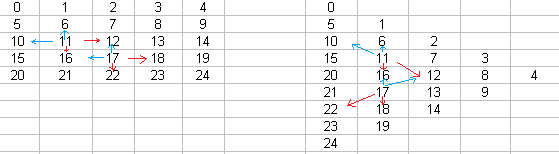
\includegraphics[width=1\textwidth]{bilder/hack.png}
  \caption{Veranschaulichung der Permutation, welche verwendet wird sowie der Verschiebung der Indexe anhand eines Beispiels. hack ist dabei blau und hack2 rot.}
  \label{fig:Bild1}
\end{figure}

\section{Methodenwahl}
Da das Gauß-Seidel-Verfahren schneller konvergiert als das Jacobi-Verfahren (siehe Abschnitt~\ref{konvergenz}) und zudem unsere parallele Implementierung des Gauß-Seidel-Verfahrens mittels Rot-Schwarz-Verfahren TODO

\end{document}
